\documentclass[aps,prb,twocolumn,nofootinbib,superscriptaddress,floatfix]{revtex4-2}
\usepackage{amsmath,amssymb,amsthm,mathtools,bm}
\usepackage{booktabs}
\usepackage{graphicx}
\usepackage{tabularx}
\usepackage[colorlinks=true,linkcolor=blue,citecolor=blue,urlcolor=blue]{hyperref}
\usepackage{microtype}

\hypersetup{
  pdftitle={Gaussian gain-loss response at a class-A dynamical domain wall},
  pdfauthor={Class-A fermionic adaptive-circuit project}
}

\graphicspath{{figures/}{../../mean_channel_lindblad_cpu_campaign/results/mean_channel_lindblad_cpu_v2_hybrid_response_production_df092e76037c014f/analysis/}}

\newcommand{\Tr}{\operatorname{Tr}}
\newcommand{\tr}{\operatorname{tr}}
\newcommand{\Gss}{G_{\mathrm{ss}}}
\newcommand{\id}{\mathbf{1}}
\newcommand{\dd}{\mathrm{d}}
\newcommand{\Diss}{\mathcal{D}}

\begin{document}

\title{Gaussian gain--loss response at a class-A dynamical domain wall}
\author{Internal campaign summary}
\affiliation{Class-A fermionic adaptive-circuit project}
\date{\today}

\begin{abstract}
This note records deterministic CPU campaign \texttt{df092e76037c014f} using
the notation of Bhuiyan, Pan, and Jian \cite{Bhuiyan2026}. The computed
generator is exactly the Gaussian sector
$\mathcal L_{\mathrm G}=\mathcal L_{\mathrm{gain}}+
\mathcal L_{\mathrm{loss}}$ of their effective cycle Lindbladian; it omits
$\mathcal L_{\mathrm{dephas.}}$ and contains neither Born trajectories nor
schedule sampling. We derive the closed equation for the two-point correlation
matrix $G$, its stationary Sylvester solution, a finite completely-positive
Strang channel, and the exact retarded response to a local density-phase
impulse. The data show wall-localized natural-occupation flow through half
occupation and oppositely oriented signed density responses at the two walls,
but also a finite mean damping gap and exponential response extinction. The
calculation therefore establishes neither a gapless full Lindbladian nor a
trajectory Lyapunov boundary mode of the projective adaptive circuit.
\end{abstract}

\maketitle
\setcounter{tocdepth}{2}
\tableofcontents

\section{Scope and bottom line}

Four spectral objects must be kept distinct. First, the auxiliary two-band
class-A Hamiltonian is used only to synthesize an overcomplete Wannier (OW)
basis. Second, the eigenvalues $\nu\in[0,1]$ of the stationary correlation
matrix $\Gss$ are natural occupations; their crossing at $\nu=1/2$
diagnoses a closing of the stationary occupation or purity gap. Third, the
positive one-particle matrix $D$ controls deterministic mean relaxation.
Fourth, the original adaptive measurement-only circuit is a random product of
record-conditioned instruments and has a distinct tangent/Lyapunov spectrum.
The present campaign computes only the second and third objects for
$\mathcal L_{\mathrm G}$, together with a finite completely-positive
discretization of that Gaussian generator.

The central result is correspondingly two-sided. At
$(\alpha_{\rm run,in},\alpha_{\rm run,out})=(1,30)$, two wall-localized occupation
branches cross $\nu=1/2$ with opposite $k_y$ slopes and the bulk occupation
gap remains approximately $1/2$. A local phase impulse produces signed density
dipoles whose positive lobes drift in opposite $y$ directions on the two
walls. Nevertheless the smallest one-particle damping rate is
$d_{\min}=0.2795656$ in the full-frame canonical case; the impulse response
decays exponentially. Stationary spectral flow and gapless dynamics are
therefore not interchangeable statements.

\section{OW bath and exact Gaussian closure}

\subsection{Auxiliary band geometry and frame operators}

Following Ref.~\cite{Bhuiyan2026}, let
$\hat c(\boldsymbol k)=(\hat c_1(\boldsymbol k),
\hat c_2(\boldsymbol k))^{\mathsf T}$. The campaign synthesizes OW states
from the auxiliary parent Hamiltonian
\begin{equation}
 \hat H_{\rm CI}(\alpha_{\rm run})=
 \sum_{\boldsymbol k}\hat c^\dagger(\boldsymbol k)
 h_{\alpha_{\rm run}}(\boldsymbol k)\hat c(\boldsymbol k)
\end{equation}
and its flattened single-particle matrix
\begin{align}
 h_{\alpha_{\rm run}}(\boldsymbol k)
 &=\widehat{\boldsymbol n}_{\alpha_{\rm run}}(\boldsymbol k)
 \cdot\boldsymbol\sigma,\nonumber\\
 \boldsymbol n_{\alpha_{\rm run}}(\boldsymbol k)
 &=\bigl(\sin k_x,\sin k_y,
 \alpha_{\rm run}-\cos k_x-\cos k_y\bigr),
 \label{eq:parent}
\end{align}
with $P_\pm(\boldsymbol k)=(\id\pm
h_{\alpha_{\rm run}}(\boldsymbol k))/2$. This run convention is sign-reversed relative to
the published parent Hamiltonian: throughout this note
\begin{equation}
 \alpha_{\rm PRR}=-\alpha_{\rm run}.
 \label{eq:alphamap}
\end{equation}
The archived labels and figures retain $\alpha_{\rm run}=1,30,\ldots$.
For each center $\boldsymbol r=(x,y)$, the code uses the \emph{uniform}
parent at its local $\alpha_{\rm run}(x)$; it never diagonalizes a spatial
domain-wall Hamiltonian. It projects the trial orbitals
$|\tau_A\rangle=(1,1)^{\mathsf T}/\sqrt2$ and
$|\tau_B\rangle=(1,-1)^{\mathsf T}/\sqrt2$ onto $P_\pm$ and Fourier transforms them
to $|W_{\boldsymbol r,\nu,\pm}\rangle$, $\nu=A,B$.

Let $\boldsymbol r'$ denote a support cell. With
\begin{align}
 M_{n_{\rm shell}}(\boldsymbol r'-\boldsymbol r)
 &=\mathbf{1}\{|\Delta x|_{\rm per},|\Delta y|_{\rm per}
 \le n_{\rm shell}\},\nonumber\\
 M_{\rm DW}(r'_x;r_x)&=\mathbf{1}\{r'_x,r_x
 \text{ lie in the same domain}\},
\end{align}
the normalized mode actually used is
\begin{equation}
 |\widetilde W_{\boldsymbol r,\nu,\pm}\rangle=
 \frac{M_{n_{\rm shell}}M_{\rm DW}
 |W_{\boldsymbol r,\nu,\pm}\rangle}
 {\|M_{n_{\rm shell}}M_{\rm DW}
 |W_{\boldsymbol r,\nu,\pm}\rangle\|}.
 \label{eq:truncatedmode}
\end{equation}
Here $M_{n_{\rm shell}}=1$ denotes the full frame, and $M_{\rm DW}=1$ when
hard wall truncation is disabled. The OW states remain nonorthogonal and
overcomplete. Define their positive frame operators
\begin{equation}
 F_\pm=\sum_{\boldsymbol r,\nu=A,B}
 |\widetilde W_{\boldsymbol r,\nu,\pm}\rangle
 \langle\widetilde W_{\boldsymbol r,\nu,\pm}|,
 \label{eq:frames}
\end{equation}
which are not projectors in general.

The canonical profile has $N_x=20$, walls at $x=5,15$, and
$\alpha_{\rm run,out}=30$. All coefficients are periodic and uniform along
$y$. Since the shell mask depends only on relative periodic displacement and
the wall mask only on $x$,
\begin{align}
 T_y|\widetilde W_{x,y,\nu,\pm}\rangle
 &=|\widetilde W_{x,y+1,\nu,\pm}\rangle,\nonumber\\
 [T_y,F_\pm]&=0,\qquad [T_y,D]=[T_y,S]=0.
 \label{eq:translation}
\end{align}
This is an exact symmetry of the deterministic generator. A fixed adaptive
trajectory or fixed noncommuting raster order has no corresponding guarantee.

Using
$\hat c_{x\sigma}(k_y)=N_y^{-1/2}\sum_y e^{-ik_y y}\hat c_{xy\sigma}$,
translation symmetry reduces every single-particle matrix to $2N_x=40$
dimensional blocks. In the published correlation convention,
\begin{equation}
 G_{x\sigma,x'\sigma'}(k_y)=\frac1{N_y}\sum_{y,y'}e^{ik_y(y-y')}
 G_{xy\sigma,x'y'\sigma'}.
 \label{eq:kyblock}
\end{equation}

\subsection{Gaussian sector of the effective Lindbladian}

The OW fermion modes and their number stabilizers are
\begin{align}
 \hat\chi_{\boldsymbol r,\nu,\pm}
 &=\sum_{\boldsymbol r',\sigma}
 \widetilde W_{\boldsymbol r,\nu,\pm}(\boldsymbol r',\sigma)
 \hat c_{\boldsymbol r',\sigma},\nonumber\\
 \hat N_{\boldsymbol r,\nu,\pm}
 &=\hat\chi_{\boldsymbol r,\nu,\pm}^\dagger
 \hat\chi_{\boldsymbol r,\nu,\pm}.
 \label{eq:owoperators}
\end{align}
Distinct OW stabilizers generally do not commute. With
\begin{equation}
 \Diss[\hat L](\hat\rho)=\hat L\hat\rho\hat L^\dagger
 -\tfrac12\{\hat L^\dagger\hat L,\hat\rho\},
\end{equation}
the campaign generator is
\begin{align}
 \mathcal L_{\rm gain}&=\bar n_{\rm a}
 \sum_{\boldsymbol r,\nu}\Diss[
 \hat\chi_{\boldsymbol r,\nu,-}^\dagger],\nonumber\\
 \mathcal L_{\rm loss}&=(1-\bar n_{\rm a})
 \sum_{\boldsymbol r,\nu}\Diss[
 \hat\chi_{\boldsymbol r,\nu,+}],\nonumber\\
 \mathcal L_{\rm G}&=\mathcal L_{\rm gain}+\mathcal L_{\rm loss}.
 \label{eq:LG}
\end{align}
It is the Gaussian part of the paper's effective generator
\begin{equation}
 \mathcal L_{\rm cycle}=\mathcal L_{\rm G}
 +\mathcal L_{\rm dephas.}.
 \label{eq:Lcycle}
\end{equation}
For reference, the omitted sector is
\begin{multline}
 \mathcal L_{\rm dephas.}=(2-\bar n_{\rm a})
 \sum_{\boldsymbol r,\nu}\Diss[\hat N_{\boldsymbol r,\nu,-}]\\
 +(1+\bar n_{\rm a})
 \sum_{\boldsymbol r,\nu}\Diss[\hat N_{\boldsymbol r,\nu,+}].
 \label{eq:omitteddephasing}
\end{multline}
That non-Gaussian many-body sector was not simulated here; neither was the
ordered projective adaptive circuit.

Fix the paper's two-point convention
\begin{equation}
 G_{ij}=\Tr(\hat\rho\,\hat c_i^\dagger\hat c_j).
 \label{eq:corrdef}
\end{equation}
The production solver stores the transposed convention, so the exact bridge is
\begin{equation}
 C_{\rm arch}=G^{\mathsf T}=G^*.
 \label{eq:archivemap}
\end{equation}
The last equality uses Hermiticity. Consequently, transposition changes
eigenvectors by complex conjugation but leaves natural occupations and spatial
weights invariant.

For $\hat G_{ij}=\hat c_i^\dagger\hat c_j$, the adjoint identity
\begin{equation}
 \Diss^\dagger[\hat L](\hat O)=\tfrac12\bigl(
 \hat L^\dagger[\hat O,\hat L]+[\hat L^\dagger,\hat O]\hat L\bigr)
 \label{eq:adjointidentity}
\end{equation}
and the canonical anticommutation relations close the dynamics exactly on
$G$. Because of Eq.~\eqref{eq:corrdef}, the OW frame enters complex
conjugated:
\begin{align}
 \dot G&=-DG-GD+S,\label{eq:correlation}\\
 D&=\tfrac12\left[\bar n_{\rm a}F_-^*
 +(1-\bar n_{\rm a})F_+^*\right],\nonumber\\
 S&=\bar n_{\rm a}F_-^*.
 \label{eq:DS}
\end{align}
For one mode this gives
$\dot g=\gamma^+(1-g)-\gamma^-g$, fixing all factors and signs.

\subsection{Stationary solution, damping, and occupation topology}

The stationary correlation matrix solves the Sylvester equation
\begin{equation}
 D\Gss+\Gss D=S.
 \label{eq:sylvester}
\end{equation}
Writing $D=U\,\mathrm{diag}(d_a)U^\dagger$ gives the explicit solution
\begin{equation}
 (U^\dagger\Gss U)_{ab}
 =\frac{(U^\dagger S U)_{ab}}{d_a+d_b}.
 \label{eq:stationarysolution}
\end{equation}
Translation along $y$ reduces this to independent $2N_x=40$ dimensional
blocks $D(k_y)$ and $G(k_y)$. A two-point perturbation obeys
\begin{equation}
 \delta G(t)=e^{-Dt}\delta G(0)e^{-Dt},
 \label{eq:homogeneous}
\end{equation}
so its elementary decay rates are sums $d_a+d_b$. The one-particle
$d_{\min}$ is therefore a stability proxy, while the correlation-sector gap begins
at $2d_{\min}$.

By contrast, the natural occupations $\nu_j(k_y)$ are eigenvalues of
$G(k_y)$. When the bulk is separated from $\nu=1/2$, one may flatten
$Q_G=\id-2\Gss$ or introduce the Gaussian modular matrix
\begin{equation}
 h_{\rm mod}=\log[(\id-\Gss)\Gss^{-1}].
\end{equation}
A branch crossing $\nu=1/2$ is a zero crossing of either classifying
representative. It says nothing by itself about a zero of $D$ or of a
trajectory Lyapunov exponent \cite{Mao2024,Lieu2020}.

\section{Finite channel and continuous limit}

The finite map is not the projective adaptive circuit. It is a
completely-positive Gaussian channel that discretizes
Eqs.~\eqref{eq:LG} and \eqref{eq:correlation}. Define
$\Gamma_{\rm gain}=\bar n_{\rm a}F_-^*$ and
$\Gamma_{\rm loss}=(1-\bar n_{\rm a})F_+^*$. A loss-only interval acts as
\begin{equation}
 \mathcal E_{\rm loss}(t):G\mapsto A_-GA_-^\dagger,\qquad
 A_-=e^{-\Gamma_{\rm loss}t/2},
\end{equation}
while a gain-only interval acts as
\begin{equation}
 \mathcal E_{\rm gain}(t):G\mapsto A_+GA_+^\dagger
 +\id-A_+A_+^\dagger,\quad A_+=e^{-\Gamma_{\rm gain}t/2}.
\end{equation}
One step of size $p$ is the ordered Strang composition
\begin{equation}
 \mathcal E_p=\mathcal E_{\rm gain}(p/2)\circ
 \mathcal E_{\rm loss}(p)\circ\mathcal E_{\rm gain}(p/2).
 \label{eq:strang}
\end{equation}
Composition acts right to left. Writing
$R_p=e^{-\Gamma_{\rm gain}p/4}$ and
$L_p=e^{-\Gamma_{\rm loss}p/2}$, the complete affine step is
\begin{align}
 \mathcal E_p(G)&=A_pGA_p^\dagger+B_p,\qquad A_p=R_pL_pR_p,\nonumber\\
 B_p&=R_pL_p(\id-R_p^2)L_pR_p+\id-R_p^2.
 \label{eq:affinestep}
\end{align}
Exact affine binary exponentiation evaluates $\mathcal E_p^{\,t/p}$ without a
long time loop. At fixed physical time, Strang splitting has global error
$O(p^2)$. This controlled comparison is why the production bundle is called
\emph{hybrid}: the continuous generator supplies the stationary state and
main response, while the finite channel verifies convergence to it.

\section{Exact response to a local density-phase impulse}

\subsection{Origin of \texorpdfstring{$\delta G$}{delta G}}

Let $P_s$ project onto the two physical orbitals at source cell
$s=(x_w,y_0)$ and let
$\hat n_s=\hat{\boldsymbol c}^{\dagger}P_s\hat{\boldsymbol c}$. The
many-body impulse
\begin{equation}
 \hat U_\epsilon=e^{-i\epsilon\hat n_s}
\end{equation}
induces the one-particle rotation
$u_\epsilon=e^{-i\epsilon P_s}$ because
$[\hat n_s,\hat{\boldsymbol c}]=-P_s\hat{\boldsymbol c}$. In the correlation
convention \eqref{eq:corrdef}, the kicked state is therefore
\begin{equation}
 G_\epsilon(0)=u_\epsilon^\dagger\Gss u_\epsilon.
 \label{eq:kickedG}
\end{equation}
The symbol $\delta G$ is simply the tangent to this one-parameter family:
\begin{align}
 G_\epsilon(t)&=\Gss+\epsilon\,\delta G(t)+O(\epsilon^2),\\
 \delta G(0)&=\left.\partial_\epsilon G_\epsilon(0)\right|_0
 =+i[P_s,\Gss].\label{eq:deltaG0}
\end{align}
It is not an extra stochastic correlator or an assumed source. Since the kick
changes the initial state but not $D$ or $S$, subtracting the stationary
equation from Eq.~\eqref{eq:correlation} cancels the affine source:
\begin{equation}
 \dot{\delta G}=-D\delta G-\delta GD.
\end{equation}
Equations~\eqref{eq:homogeneous} and \eqref{eq:deltaG0} then give
\begin{equation}
 \boxed{\delta G(t)=+i\,e^{-Dt}[P_s,\Gss]e^{-Dt}.}
 \label{eq:exactdeltaG}
\end{equation}
For a density probe $P_r$,
\begin{equation}
 \boxed{\chi_{rs}(t)=+i\theta(t)\tr\!\left[
 P_r e^{-Dt}[P_s,\Gss]e^{-Dt}\right].}
 \label{eq:response}
\end{equation}
Because local density projectors commute,
$\chi_{rs}(0)=+i\tr([P_r,P_s]\Gss)=0$: the kick initially rotates
coherences, and the dissipative propagator subsequently converts them into
density.

The finite central difference is also analytic. Since $P_s^2=P_s$,
\begin{equation}
 \frac{G_{+\epsilon}(0)-G_{-\epsilon}(0)}{2\epsilon}
 =+i\,\frac{\sin\epsilon}{\epsilon}[P_s,\Gss].
 \label{eq:sinc}
\end{equation}
Thus $\epsilon=10^{-3}$ merely multiplies the derivative by
$\operatorname{sinc}\epsilon=1-O(10^{-7})$; no pair of numerical trajectory
simulations is required.

\subsection{Spectral, frequency, and momentum representations}

In the $D$ eigenbasis, Eq.~\eqref{eq:response} becomes
\begin{equation}
 \chi_{rs}(t)=+i\theta(t)\sum_{a,b}e^{-(d_a+d_b)t}
 \langle b|P_r|a\rangle\langle a|[P_s,\Gss]|b\rangle.
 \label{eq:spectralresponse}
\end{equation}
With Fourier convention $\int_0^\infty\dd t\,e^{i\omega t}$,
\begin{equation}
 \chi_{rs}(\omega)=+i\sum_{a,b}
 \frac{\langle b|P_r|a\rangle\langle a|[P_s,\Gss]|b\rangle}
 {d_a+d_b-i\omega}.
 \label{eq:frequencyresponse}
\end{equation}
All mean-response poles are therefore at $\omega=-i(d_a+d_b)$. A
half-occupation crossing of $\Gss$ does not create a zero-frequency pole when
$d_{\min}>0$.

For a source at $y_0$ and a wall-window probe at $y$, let $p_s,p_w$ be their
$x$-orbital projectors and $r=y-y_0$. Exact $y$-translation symmetry gives
\begin{multline}
 \chi_w(r,t)=+\frac{i}{N_y^2}\sum_{k,q}e^{i(k-q)r}\\
 \times\tr\!\left[p_w e^{-D(k)t}
 \bigl(p_sG(q)-G(k)p_s\bigr)e^{-D(q)t}\right].
 \label{eq:kyresponse}
\end{multline}
The heatmap is a direct finite evaluation of Eq.~\eqref{eq:kyresponse}.
There is no continuous-time integration.

\subsection{Rank-four implementation}

Writing $P_s=EE^\dagger$ with two source-orbital columns and
$A(t)=e^{-Dt}$, define $X=AE$ and $Y=A\Gss E$. Then
\begin{align}
 \delta G(t)&=+i(XY^\dagger-YX^\dagger),\nonumber\\
 \delta G_{ii}(t)&=+2\,\mathrm{Im}
 \sum_{\sigma=1}^2Y_{i\sigma}X^*_{i\sigma}.
 \label{eq:rankfour}
\end{align}
After applying Eq.~\eqref{eq:archivemap}, the code propagates only $E$ and
$\Gss E$ through momentum blocks and uses Eq.~\eqref{eq:rankfour}; it never
materializes a kicked correlation history. In particular,
$\delta G_{ii}=\delta(C_{\rm arch})_{ii}$, so the plotted density response is
unchanged by the convention migration.
This is an exact Gaussian Kubo impulse response
\cite{Albert2016,Venuti2016}, not Monte Carlo sampling.

\section{Campaign design and provenance}

\begin{table*}[t]
\caption{Production design. Full frame denotes
$n_{\rm shell}=\mathrm{None}$. All $\alpha$ values are $\alpha_{\rm run}$
from Eq.~\eqref{eq:alphamap}. The static sweep keeps a geometric
$\alpha_{\rm run}$ interface; for $\alpha_{\rm run,in}>2$ both regions are
topologically trivial even though the spatial step remains.}
\label{tab:design}
\begin{tabularx}{\textwidth}{@{}>{\raggedright\arraybackslash}p{0.17\textwidth}X@{}}
\toprule
Run identity & ID \texttt{df092e76037c014f}; 66/66 cases complete; complex128 CPU; 48 workers; one BLAS thread each.\\
\midrule
Main geometry & $N_x=20$; periodic $y$; canonical walls $x=5,15$; $\alpha_{\rm run,out}=30$; $\bar n_{\rm a}=1/2$; maximally mixed initialization.\\
Static scan & $N_y=64$; $\alpha_{\rm run,in}=1,1.5,1.75,1.875,2.125,2.25,2.5,3$; $n_{\rm shell}=1,2,\mathrm{None}$; \texttt{domain\_wall=True}; \texttt{dw\_truncation=True}.\\
Response endpoint & $\alpha_{\rm run,in}=1$; $N_y=32,48,64$; all three shells; truncation on and off; $\epsilon=10^{-3}$; $t\in[0,N_y/2]$ in steps $0.25$; velocity fit $2\le t\le0.375N_y$.\\
Finite channel & $p=1,1/2,1/4,1/8,1/16$ at fixed physical time; exact affine powers of the completely-positive Strang step.\\
Controls & Uniform topological and trivial geometries; $\bar n_{\rm a}=0.45,0.55$; empty and filled initial states; legacy wall rule; separate $4\times6$ dephasing-closure checks.\\
Storage contract & Zero trajectories and schedule samples; no final correlation matrix or history; compact selected-observable NPZ plus JSON metadata and checksums.\\
\bottomrule
\end{tabularx}
\end{table*}

The manifest records complete SHA-256 hashes for the solver and configuration;
their identifying prefixes are \texttt{3efc79ee1434} and
\texttt{aa2956995cac}. Momentum-resolved arrays were archived by policy only
for the full frame. Figure~\ref{fig:shell-spectrum} therefore reconstructs the
shell-one block from the pinned solver without altering the production archive.

\section{Results}

\subsection{Wall occupation spectral flow}

For every saved momentum block the scatter points in Fig.~\ref{fig:shell-spectrum}
are defined by
\begin{equation}
 G_{\rm ss}(k_y)|\phi_j(k_y)\rangle=\nu_j(k_y)|\phi_j(k_y)\rangle.
 \label{eq:occupationeigenproblem}
\end{equation}
Let $\mathcal W_a=\{x_a-1,x_a,x_a+1\}$ be the three-column window around
wall $a$. Its mode weight is
\begin{equation}
 W_j^{(a)}(k)=\sum_{x\in\mathcal W_a,\sigma}
 |\phi_{j,x\sigma}(k)|^2.
 \label{eq:wallweight}
\end{equation}
Among modes with $W_j^{(a)}\ge0.25$, the colored branch is selected separately
at each $k$ by
\begin{equation}
 j_a(k)=\arg\min_j\left\{|\nu_j(k)-\tfrac12|
 +0.02[1-W_j^{(a)}(k)]\right\}.
 \label{eq:branchselector}
\end{equation}
If no mode passes the threshold, the maximum-weight mode is used. The displayed
slope $s_a$ is the ordinary least-squares coefficient in
$\nu_{j_a(k)}=s_ak+b_a$ for
\begin{equation}
 |k|\le k_c,\qquad
 k_c=\max\!\left(2.5\frac{2\pi}{N_y},0.22\right).
 \label{eq:slopewindow}
\end{equation}
This selector is not global overlap tracking and is not itself a topological
index. At the exact $k=0$ degeneracy the eigensolver may rotate the two wall
states into each other.

\begin{figure*}[t]
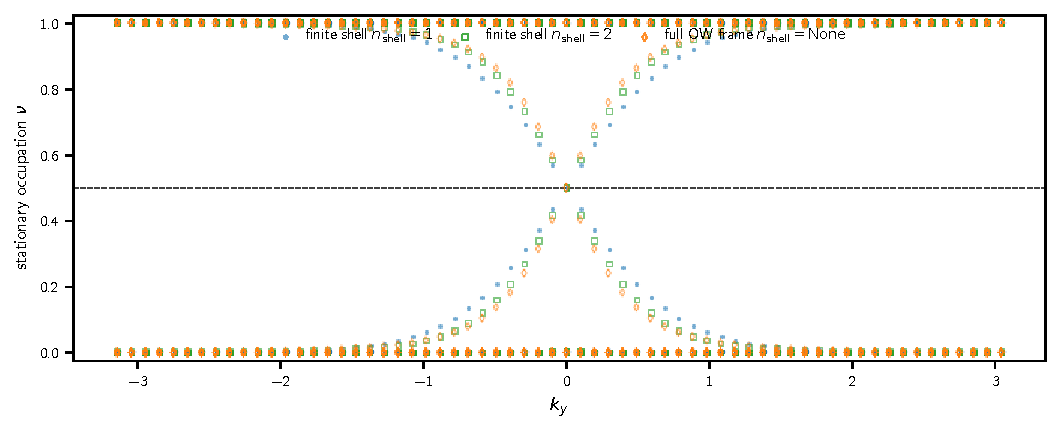
\includegraphics[width=0.98\textwidth]{overlaid_finite_shell_ky_occupation_spectrum.pdf}
\caption{Stationary $k_y$-resolved natural occupations at
$(\alpha_{\rm run,in},\alpha_{\rm run,out})=(1,30)$ with domain-wall truncation.
Every eigenvalue of $G_{\rm ss}(k_y)$ is shown without branch-selection or fit
overlays: filled blue circles denote $n_{\rm shell}=1$, open green squares
denote $n_{\rm shell}=2$, and open orange diamonds denote the full OW frame.
These are natural occupations of the mixed steady state of $\mathcal L_{\rm G}$.
The three spectra largely coincide at $\nu=0,1$; their visible difference is
concentrated in the wall branches crossing $\nu=1/2$, which become successively
steeper as the retained OW range increases.}
\label{fig:shell-spectrum}
\end{figure*}

For the canonical full-frame $N_y=64$ case,
\begin{align}
 \min_{k,j}|\nu_j(k)-\tfrac12|&=2.22\times10^{-16},\nonumber\\
 \Delta_{\rm bulk}&=0.49999999993.
\end{align}
The selected slopes are $\partial_{k_y}\nu_w=\pm0.949605$, and the stationary
Gaussian entropy is $S_G/N_y=0.317152$. The shell-one result remains sharply
distinguished: its half gap is $3.33\times10^{-10}$, bulk gap $0.496999$, and
selected wall slopes $\pm0.659914$. Shell two is intermediate, with slopes
$\pm0.823598$. Thus finite $n_{\rm shell}$ has little visible effect on the
many eigenvalues already pinned exponentially close to $0$ or $1$, but it
systematically reduces the wall-branch slope and broadens the crossing in
momentum. Uniform topological and uniform trivial
controls have half gaps $0.4969$--$0.5$ and no wall response.

The four alpha-scan panels use the following estimators. With
$\mathcal W=\mathcal W_1\cup\mathcal W_2$ and
$W_j^{\mathcal W}=\sum_{x\in\mathcal W,\sigma}|\phi_{j,x\sigma}|^2$,
\begin{align}
 \Delta_{1/2}&=\min_{k,j}|\nu_j(k)-\tfrac12|,\nonumber\\
 \Delta_{\rm bulk}&=\min_{k,j:\,W_j^{\mathcal W}(k)<0.25}
 |\nu_j(k)-\tfrac12|,\label{eq:alphagaps}\\
 \frac{S_G}{N_y}&=-\frac1{N_y}\sum_{k,j}
 [\nu_j\ln\nu_j+(1-\nu_j)\ln(1-\nu_j)].
 \label{eq:entropyestimator}
\end{align}
Thus ``bulk'' is a wall-weight exclusion within the same domain-wall state,
not a separate uniform calculation, and $S_G/N_y$ is entropy per circumference,
not per site. For the localization panel let $\mathcal M$ be the $2N_y$ pairs
$(k,j)$ closest to half occupation and define
\begin{equation}
 p_x=\frac1{|\mathcal M|}\sum_{(k,j)\in\mathcal M,\sigma}
 |\phi_{j,x\sigma}(k)|^2,\qquad
 \mathcal L_{\rm mid}=\frac{\sum_{x\in\mathcal W}p_x}{\sum_xp_x}.
 \label{eq:midgaplocalization}
\end{equation}
Finally, if $D(k)|u_a(k)\rangle=d_a(k)|u_a(k)\rangle$, a correlation
eigenoperator decays at
\begin{equation}
 \gamma_{ab}(k)=d_a(k)+d_b(k),\qquad
 \gamma_{\min}=\min_{\gamma_{ab}>10^{-12}}\gamma_{ab}.
 \label{eq:correlationrate}
\end{equation}
The lower-right panel plots $\gamma_{\min}$; at the canonical endpoint it is
$2d_{\min}=0.5591313$, not a Hamiltonian excitation gap.

\begin{figure*}[t]
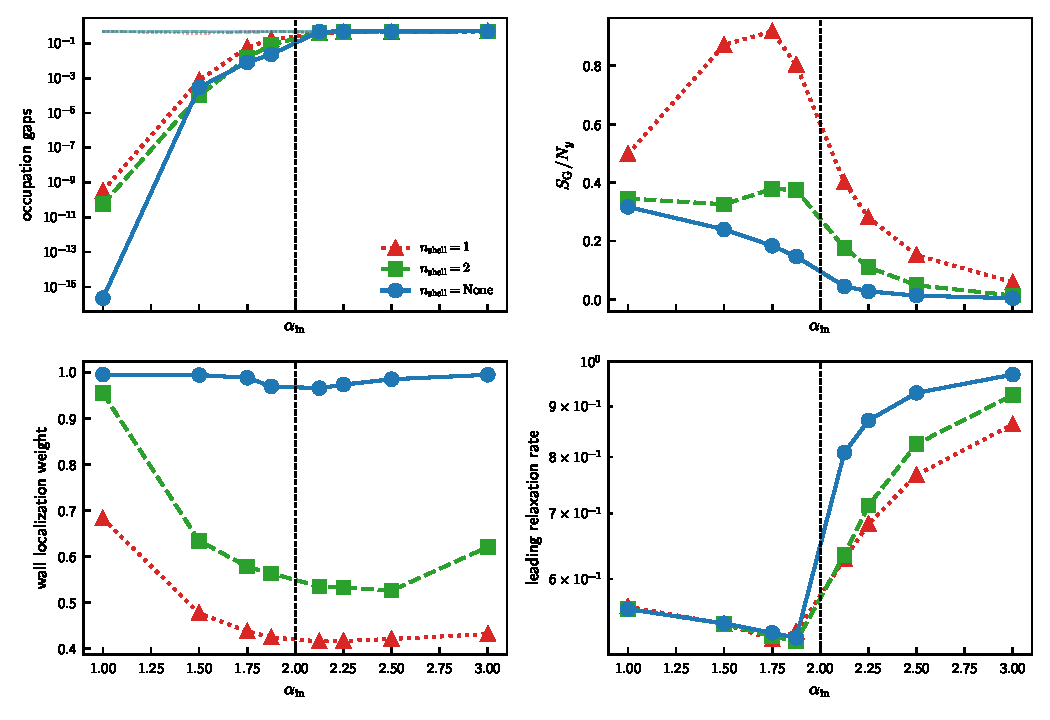
\includegraphics[width=0.98\textwidth]{appendix_static_alpha_scan.pdf}
\caption{Static $\alpha_{\rm run,in}$ sweep at $N_y=64$, with
$\alpha_{\rm run,out}=30$, the geometric interface present, and domain-wall
truncation on. The archived graphic abbreviates $\alpha_{\rm run,in}$ as
$\alpha_{\rm in}$; Eq.~\eqref{eq:alphamap} gives the PRR sign convention.
The dashed line marks the run-convention parent transition $\alpha_{\rm run}=2$.
Top left: global half-occupation gap and bulk reference. Top right:
stationary Gaussian entropy per circumference. Bottom left: localization
weight $\mathcal L_{\rm mid}$. Bottom right: smallest positive correlation-sector
decay rate $\gamma_{\min}$. The dashed line is only a parent-model reference:
$\alpha_{\rm run}=2$ itself was not sampled.}
\label{fig:alpha-scan}
\end{figure*}

Figure~\ref{fig:alpha-scan} tests whether the wall feature follows the phase
mismatch rather than the mere spatial step. For shell one the half gap grows
from $3.33\times10^{-10}$ at $\alpha_{\rm run,in}=1$ to
$7.39\times10^{-4},0.0593,0.1719$ at $1.5,1.75,1.875$, then to $0.3935$ at
$2.125$ and $0.4933$ at $3$. The full-frame gap changes from
$2.22\times10^{-16}$ at $1$ to $0.0238$ at $1.875$, $0.4802$ at $2.125$,
and $0.49946$ at $3$. Finite shells smear the approach to the parent
transition; the main qualitative change remains tied to loss of the
topological mismatch.

\subsection{What was already known about such spectra}

Chiral-looking eigenvalue branches of a mixed Gaussian state are an established
open-system idea, although the present OW domain-wall realization is different.
For a state with correlation matrix $G$, the purity or modular representative
$Q_G=\id-2G$ has the same eigenvectors and maps the occupation midpoint
$\nu=1/2$ to zero. Budich and Diehl formalized topology under precisely such
spectral constraints on density matrices \cite{Budich2015}; the modular-band
and purity-gap formulation was developed into an observable mixed-state
geometric phase by Bardyn \emph{et al.} \cite{Bardyn2018}. Bardyn
\emph{et al.} then formulated dissipative bulk--edge correspondence in terms of
two independent objects: an edge can close the steady-state purity gap, the
damping gap, or both \cite{Bardyn2013}. For two-dimensional class-A Gaussian
Chern states, Goldstein explicitly discussed topological edge modes of the
single-particle density matrix and simultaneously proved restrictions on
finite-range, finite-rate preparation of pure Chern states
\cite{Goldstein2019}.

Thus Fig.~\ref{fig:shell-spectrum} has a clear precedent: it is the mixed-state
analogue of a Chern edge spectrum, with $\nu-1/2$ replacing energy. What is
\emph{not} inherited is a Hamiltonian group velocity. Shavit and Goldstein
showed in dissipatively prepared Chern states that edge-current confinement and
the relation between the density-matrix Chern number and Hall conductance can
fail, and that a physical current requires additional dynamical structure
\cite{Shavit2020}. Our opposite occupation slopes and signed-kick orientations
are consequently suggestive state-level chirality, while the finite $D$ gap
demonstrates that they are not undamped mean-channel edge modes. Chiral
topological response has been derived for driven-open Chern states under
stronger purity and particle-number-conservation assumptions
\cite{Tonielli2020}; the gain/loss bath here satisfies neither assumption.

\subsection{Directional but extinguished density response}

Figure~\ref{fig:response} contains two distinct impulse experiments. For panel
$a$, both source orbitals are kicked at that panel's wall,
\begin{align}
 P_{a,0}&=\sum_\sigma|x_a,y_0,\sigma\rangle
 \langle x_a,y_0,\sigma|,\nonumber\\
 \delta G_a^{(\epsilon)}(t)&=+i\,\operatorname{sinc}(\epsilon)
 e^{-Dt}[P_{a,0},\Gss]e^{-Dt}.
 \label{eq:wallkick}
\end{align}
The sinc factor is the exact central-difference factor in
Eq.~\eqref{eq:sinc}. The real-space response and plotted three-column profile
are
\begin{align}
 \chi_a(x,r,t)&=\sum_\sigma
 [\delta G_a^{(\epsilon)}(t)]_{x,y_0+r,\sigma;x,y_0+r,\sigma},\nonumber\\
 \chi_a^{\rm wall}(r,t)&=\sum_{x\in\mathcal W_a}\chi_a(x,r,t).
 \label{eq:wallprofile}
\end{align}
The full-density norm and wall retention are, respectively,
\begin{align}
 \mathcal N_a(t)&=\sum_{x,r}|\chi_a(x,r,t)|,\nonumber\\
 \mathcal R_a(t)&=\frac{\sum_{x\in\mathcal W_a,r}|\chi_a(x,r,t)|}
 {\mathcal N_a(t)}.
 \label{eq:normretention}
\end{align}
On the periodic ring define
$\widetilde r=((r+N_y/2)\bmod N_y)-N_y/2$ and $[z]_+=\max(z,0)$.
The white points in the figure are the positive-lobe center
\begin{equation}
 y_{+,a}(t)=\frac{\sum_r\widetilde r[\chi_a^{\rm wall}(r,t)]_+}
 {\sum_r[\chi_a^{\rm wall}(r,t)]_+}.
 \label{eq:positivecenter}
\end{equation}
The yellow line is its ordinary least-squares fit over
$2\le t\le0.375N_y$, retaining times for which
$\mathcal N_a(t)>\max(10^{-8}\mathcal N_{a,\max},10^{-15})$. Its $R^2$ is
deterministic fit quality, not a statistical confidence interval.

\begin{figure*}[t]
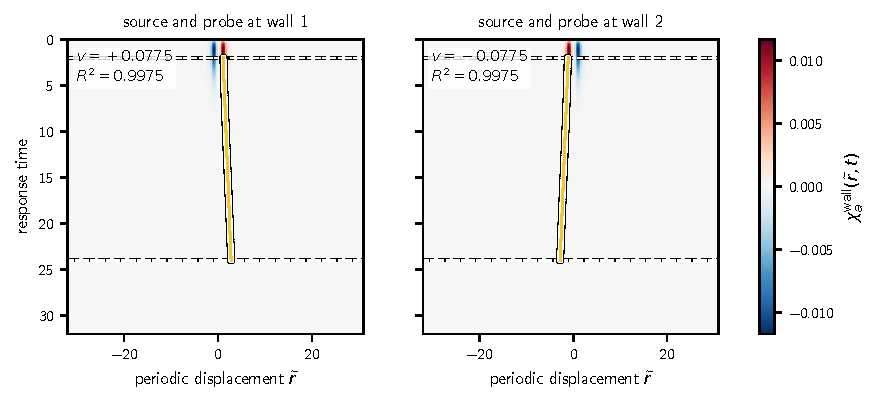
\includegraphics[width=0.98\textwidth]{directional_density_response_estimators.pdf}
\caption{Exact continuous-time response $\chi_a^{\rm wall}$ for the canonical
full-frame $N_y=64$ endpoint. Each panel uses a separate kick placed at its
named wall. White points show Eq.~\eqref{eq:positivecenter}, yellow lines show
the velocity fit, and horizontal dashed lines bound its time window. The
opposite signed-dipole orientations coexist with exponential extinction.}
\label{fig:response}
\end{figure*}

The response begins at numerical zero in density, grows as coherences rotate
into diagonal weight, reaches an $L^1$ norm $0.02673$ at $t=1.25$, and then
falls to $7.61\times10^{-4}$ at $t=8$, $4.96\times10^{-6}$ at $t=16$, and
$3.15\times10^{-10}$ at $t=32$. Its final norm is $1.18\times10^{-8}$ of
the peak. During the fit the response remains essentially at its source wall
(retention $>0.999$), so decay is not caused by leakage across the slab.

The centers of the positive lobes fit
\begin{equation}
 v_1=+0.077455,\qquad v_2=-0.077455,\qquad R^2=0.99753
\end{equation}
for the canonical full frame. These are velocities of a signed, decaying
shape, not Hamiltonian group velocities and not quantized charge transport.
Absolute right/left weight asymmetry is zero; orientation resides in the
signed dipole. Because $D$ is Hermitian positive, asymmetric spectral
filtering and complex chiral matrix elements can move this signed center
without producing an oscillatory real-time edge quasiparticle.

The left panel of Fig.~\ref{fig:convergence} plots these raw OLS slopes against
$1/N_y$; no thermodynamic extrapolation is performed. Solid curves enforce
Eq.~\eqref{eq:truncatedmode}'s domain-wall mask, while dashed curves allow OW
support across the wall. The right panel compares finite and continuous
responses at $t_f=N_y/2$ using
\begin{equation}
 E_\chi(p)=\frac{\|\chi_p(t_f)-\chi_{\rm cont}(t_f)\|_2}
 {\|\chi_{\rm cont}(t_f)\|_2}.
 \label{eq:responseerror}
\end{equation}
Here $\chi_p$ is evaluated with the homogeneous factor $A_p^{t_f/p}$ of the
affine channel, obtained by exact binary exponentiation. The separately quoted
state error at $t_G=2N_y$ is
\begin{equation}
 E_G(p)=\frac{\|G_p(t_G)-G_{\rm cont}(t_G)\|_F}
 {\|G_{\rm cont}(t_G)\|_F},\qquad t_G=2N_y.
 \label{eq:stateerror}
\end{equation}

\begin{figure*}[t]
\begin{minipage}[t]{0.49\textwidth}
\centering
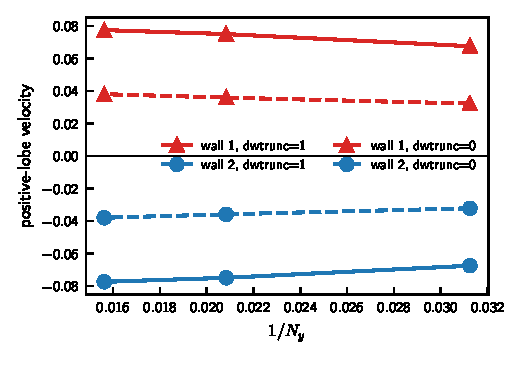
\includegraphics[width=\linewidth]{response_velocity_size_check.pdf}
\end{minipage}\hfill
\begin{minipage}[t]{0.49\textwidth}
\centering
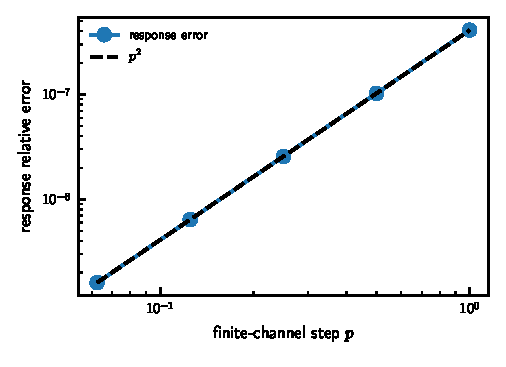
\includegraphics[width=\linewidth]{response_channel_to_continuous.pdf}
\end{minipage}
\caption{Left: positive-lobe velocities for $N_y=32,48,64$ in full-frame
wall calculations, with hard domain-wall truncation (solid) and without it
(dashed). The two wall orientations remain opposite; truncation strengthens
the measured drift. These are raw size points, not an extrapolation. Right:
$E_\chi(p)$ from Eq.~\eqref{eq:responseerror}; the dashed $p^2$ guide is
anchored at the smallest saved $p$.}
\label{fig:convergence}
\end{figure*}

At $N_y=32,48,64$, canonical full-frame speeds are respectively
$0.06753,0.07499,0.07745$ in magnitude; without hard wall truncation they are
$0.03222,0.03594,0.03803$. At $N_y=64$ with truncation, the magnitudes
increase systematically from shell one to shell two to full frame:
$0.05104,0.06890,0.07745$. The orientation is robust, while its magnitude is
not universal.

\subsection{Convergence, controls, and numerical validation}

For the canonical full-frame case, the finite-channel state error relative to
the continuous solution decreases from $6.32\times10^{-4}$ at $p=1$ to
$2.49\times10^{-6}$ at $p=1/16$; the corresponding response error decreases
from $4.11\times10^{-7}$ to $1.60\times10^{-9}$. Log--log fits give orders
$1.99697$ for $E_G$ and $2.00088$ for $E_\chi$, verifying global $O(p^2)$
convergence. Empty, filled, and maximally mixed initial
conditions converge to the same stationary observables. Biasing the bath to
$\bar n_{\rm a}=0.45$ or $0.55$ symmetrically opens the canonical full-frame
half-occupation gap to $0.04755$.

All 66 manifest cases completed and all 132 case-file checksums match. Across
primary Gaussian cases, the maximum stationary relative residual was
$3.98\times10^{-15}$, the maximum frame norm error $4.88\times10^{-15}$,
the recorded translation residual zero, the largest continuous-correlation
physicality violation $6.44\times10^{-15}$, and the largest finite-channel
physicality violation $2.83\times10^{-13}$. The small $4\times6$ dephasing
cases are historical physicality controls from a different bath family and
are not evidence for the primary gain/loss response.

\section{Interpretation and limitations}

The calculation is a concrete quasi-free instance of Lindbladian Kubo response
\cite{Albert2016,Venuti2016}. For an impulsive Hamiltonian perturbation
$-i[\hat n_s,\mathord\cdot]$, Eq.~\eqref{eq:response} is the decaying-sector response of a
unique stationary state. A sustained or adiabatic flux perturbation would
instead require perturbing $D$ and $S$ and solving
\begin{equation}
 D\delta G+\delta G D-i\omega\delta G
 =\delta S-\delta D\,\Gss-\Gss\,\delta D,
\end{equation}
with a carefully defined open-system current; such flux definitions are not
unique in general \cite{Avron2012}. The local kick used here is nevertheless
well-defined and its full response is given by
Eqs.~\eqref{eq:response}--\eqref{eq:kyresponse}.

The campaign establishes three facts: a stationary wall occupation crossing,
wall-confined oppositely oriented signed response, and a finite mean damping
gap. It does not establish a gapless Lindbladian pole, a quantized Hall
coefficient, physical chirality of individual adaptive trajectories, or a
wall-localized zero Lyapunov exponent. Those require record-resolved tangent
or Choi transfer data, system-size scaling after removing exact null sectors,
and a directed probe propagated through the same Born record. The present
mean calculation is therefore a controlled baseline and an analytic
counterexample to conflating stationary correlation-matrix topology with dynamical
gaplessness.

\section{Reproduction checklist}

The authoritative run root is the production directory named in
Table~\ref{tab:design}; its manifest status is \texttt{complete}. The note
uses the archived analysis PDFs directly. Figures~\ref{fig:shell-spectrum} and
\ref{fig:response} are regenerated by
\texttt{make\_supplementary\_figures.py}, which imports the pinned campaign
solver, reconstructs $G(k_y)=C_{\rm arch}^{\mathsf T}(k_y)$ for shell one and
the full frame, annotates the
archived response, and verifies all 132 production checksums before and after
plotting. It leaves all production files untouched. Compilation uses
RevTeX~4.2 in double-column PRB format. The acceptance gate for this working
note is a clean PDF containing fewer than ten pages.

\begin{thebibliography}{15}
\bibitem{Bhuiyan2026}
A.~Bhuiyan, H.~Pan, and C.-M.~Jian,
Free-fermion dynamics with measurements: Topological classification and
adaptive preparation of topological states,
Phys. Rev. Research \textbf{8}, 023147 (2026).
\bibitem{Lindblad1976}
G.~Lindblad, On the generators of quantum dynamical semigroups,
Commun. Math. Phys. \textbf{48}, 119 (1976).
\bibitem{Albert2016}
V.~V.~Albert, B.~Bradlyn, M.~Fraas, and L.~Jiang,
Geometry and response of Lindbladians,
Phys. Rev. X \textbf{6}, 041031 (2016).
\bibitem{Venuti2016}
L.~Campos Venuti and P.~Zanardi,
Dynamical response theory for driven-dissipative quantum systems,
Phys. Rev. A \textbf{93}, 032101 (2016).
\bibitem{Avron2012}
J.~E.~Avron, M.~Fraas, and G.~M.~Graf,
Adiabatic response for Lindblad dynamics,
J. Stat. Phys. \textbf{148}, 800 (2012).
\bibitem{Mao2024}
L.~Mao, F.~Yang, and H.~Zhai,
Symmetry-preserving quadratic Lindbladian and dissipation-driven topological
transitions in Gaussian states,
Rep. Prog. Phys. \textbf{87}, 070501 (2024).
\bibitem{Lieu2020}
S.~Lieu, M.~McGinley, and N.~R.~Cooper,
Tenfold way for quadratic Lindbladians,
Phys. Rev. Lett. \textbf{124}, 040401 (2020).
\bibitem{Budich2015}
J.~C.~Budich and S.~Diehl,
Topology of density matrices,
Phys. Rev. B \textbf{91}, 165140 (2015).
\bibitem{Bardyn2018}
C.-E.~Bardyn, L.~Wawer, A.~Altland, M.~Fleischhauer, and S.~Diehl,
Probing the topology of density matrices,
Phys. Rev. X \textbf{8}, 011035 (2018).
\bibitem{Bardyn2013}
C.-E.~Bardyn, M.~A.~Baranov, C.~V.~Kraus, E.~Rico, A.~Imamo\u{g}lu,
P.~Zoller, and S.~Diehl,
Topology by dissipation,
New J. Phys. \textbf{15}, 085001 (2013).
\bibitem{Goldstein2019}
M.~Goldstein,
Dissipation-induced topological insulators: A no-go theorem and a recipe,
SciPost Phys. \textbf{7}, 067 (2019).
\bibitem{Shavit2020}
G.~Shavit and M.~Goldstein,
Topology by dissipation: Transport properties,
Phys. Rev. B \textbf{101}, 125412 (2020).
\bibitem{Tonielli2020}
F.~Tonielli, J.~C.~Budich, A.~Altland, and S.~Diehl,
Topological field theory far from equilibrium,
Phys. Rev. Lett. \textbf{124}, 240404 (2020).
\end{thebibliography}

\end{document}
